\documentclass[anonymous, sigconf]{acmart}
\settopmatter{printacmref=false}
%%
%% \BibTeX command to typeset BibTeX logo in the docs
\AtBeginDocument{%
  \providecommand\BibTeX{{%
    Bib\TeX}}}

% %% Rights management information.  This information is sent to you
% %% when you complete the rights form.  These commands have SAMPLE
% %% values in them; it is your responsibility as an author to replace
% %% the commands and values with those provided to you when you
% %% complete the rights form.
% \setcopyright{acmlicensed}
% \copyrightyear{2018}
% \acmYear{2018}
\acmDOI{}
%% These commands are for a PROCEEDINGS abstract or paper.
\acmConference[ASP-DAC '27]
{32nd Asia and South Pacific Design Automation Conference}
{January 25--28, 2027}
{Tokyo, Japan}
% %
% %  Uncomment \acmBooktitle if the title of the proceedings is different
% %  from ``Proceedings of ...''!
% %
% %\acmBooktitle{Woodstock '18: ACM Symposium on Neural Gaze Detection,
% %  June 03--05, 2018, Woodstock, NY}
\acmISBN{}


%%
%% Submission ID.
%% Use this when submitting an article to a sponsored event. You'll
%% receive a unique submission ID from the organizers
%% of the event, and this ID should be used as the parameter to this command.
%%\acmSubmissionID{123-A56-BU3}

%%
%% For managing citations, it is recommended to use bibliography
%% files in BibTeX format.
%%
%% You can then either use BibTeX with the ACM-Reference-Format style,
%% or BibLaTeX with the acmnumeric or acmauthoryear sytles, that include
%% support for advanced citation of software artefact from the
%% biblatex-software package, also separately available on CTAN.
%%
%% Look at the sample-*-biblatex.tex files for templates showcasing
%% the biblatex styles.
%%
%%
%% The majority of ACM publications use numbered citations and
%% references.  The command \citestyle{authoryear} switches to the
%% "author year" style.
%%
%% If you are preparing content for an event
%% sponsored by ACM SIGGRAPH, you must use the "author year" style of
%% citations and references.
%% Uncommenting
%% the next command will enable that style.
%%\citestyle{acmauthoryear}


%%
%% end of the preamble, start of the body of the document source.
\begin{document}

%%
%% The "title" command has an optional parameter,
%% allowing the author to define a "short title" to be used in page headers.
\title{ZhuLong: Execution-Grounded LLM Agent for EDA Scripting with Offline API Self-Exploration}

%%
%% The "author" command and its associated commands are used to define
%% the authors and their affiliations.
%% Of note is the shared affiliation of the first two authors, and the
%% "authornote" and "authornotemark" commands
%% used to denote shared contribution to the research.
\author{Ben Trovato}
\authornote{Both authors contributed equally to this research.}
\email{trovato@corporation.com}
\orcid{1234-5678-9012}
\author{G.K.M. Tobin}
\correspondingauthor
\authornotemark[1]
\email{webmaster@marysville-ohio.com}
\affiliation{%
  \institution{Institute for Clarity in Documentation}
  \city{Dublin}
  \state{Ohio}
  \country{USA}
}

\author{Lars Th{\o}rv{\"a}ld}
\affiliation{%
  \institution{The Th{\o}rv{\"a}ld Group}
  \city{Hekla}
  \country{Iceland}}
\email{larst@affiliation.org}

\author{Valerie B\'eranger}
\affiliation{%
  \institution{Inria Paris-Rocquencourt}
  \city{Rocquencourt}
  \country{France}
}

\author{Aparna Patel}
\affiliation{%
 \institution{Rajiv Gandhi University}
 \city{Doimukh}
 \state{Arunachal Pradesh}
 \country{India}}

\author{Huifen Chan}
\affiliation{%
  \institution{Tsinghua University}
  \city{Haidian Qu}
  \state{Beijing Shi}
  \country{China}}

\author{Charles Palmer}
\affiliation{%
  \institution{Palmer Research Laboratories}
  \city{San Antonio}
  \state{Texas}
  \country{USA}}
\email{cpalmer@prl.com}

\author{John Smith}
\affiliation{%
  \institution{The Th{\o}rv{\"a}ld Group}
  \city{Hekla}
  \country{Iceland}}
\email{jsmith@affiliation.org}

\author{Julius P. Kumquat}
\correspondingauthor
\affiliation{%
  \institution{The Kumquat Consortium}
  \city{New York}
  \country{USA}}
\email{jpkumquat@consortium.net}

%%
%% By default, the full list of authors will be used in the page
%% headers. Often, this list is too long, and will overlap
%% other information printed in the page headers. This command allows
%% the author to define a more concise list
%% of authors' names for this purpose.
\renewcommand{\shortauthors}{Trovato et al.}

%%
%% The abstract is a short summary of the work to be presented in the
%% article.
\begin{abstract}
    EDA scripting with tool-specific, often undocumented APIs remains a long-tail 
    bottleneck that existing LLMs fail to address. This paper presents 
    \textbf{ZhuLong}, an execution-grounded LLM coding agent for PyAether and 
    SKILL that combines API retrieval, documentation inspection, and sandbox 
    execution via unified MCP tools, augmented by an offline \textbf{API 
    self-exploration mechanism} that infers undocumented API behaviors through 
    counterfactual experimentation.
    % 使用工具特定且常无文档的EDA API进行脚本编写，仍是现有LLM无法解决的
    % 长尾瓶颈。本文提出\textbf{ZhuLong}，一个面向PyAether和SKILL的执行驱动
    % LLM代码智能体，通过统一的MCP工具组合API检索、文档查阅和沙盒执行，
    % 并辅以离线\textbf{API自探索机制}，通过反事实实验推断未文档化的API行为。
    
    We evaluate ZhuLong on \textbf{EDA-Eval-PyAether}, a benchmark of 158
    real-world tasks with assertion-based execution, where the complete system
    achieves \textbf{78.5\%} Pass@1 in the commercial Empyrean Aether
    environment, substantially outperforming a pure LLM baseline (\textbf{23.6\%}). Ablation studies identify sandbox execution as the dominant
    performance driver (41.2 pp drop when removed), with the self-exploration
    mechanism contributing an additional 3.2 pp accuracy gain and a 22.1\%
    reduction in per-task tool calls. On 20 interactive tasks involving unsaved
    layouts and schematics, ZhuLong achieves 60.0\% Pass@1 for PyAether and
    50.0\% for SKILL. 
    % 我们在\textbf{EDA-Eval-PyAether}上评估ZhuLong，该基准包含158个真实任务，
    % 采用基于断言的执行验证，完整系统在商业Empyrean Aether环境中达到
    % \textbf{78.5\%}的Pass@1，显著优于纯LLM基线（\textbf{23.6\%}）。消融实验表明，沙盒执行是性能提升的主导因素
    % （移除后下降41.2个百分点），自探索机制在贡献额外3.2个百分点准确率提升的
    % 同时，将每任务工具调用次数减少22.1\%。在20个涉及未保存版图和原理图的
    % 交互任务中，ZhuLong在PyAether上达到60.0\% Pass@1，在SKILL上达到
    % 50.0\% Pass@1。
\end{abstract}

\keywords{LLM Agents for EDA, EDA Scripting, Code Generation, Sandbox Execution, API Self-Exploration}

% %%
% %% The code below is generated by the tool at http://dl.acm.org/ccs.cfm.
% %% Please copy and paste the code instead of the example below.
% %%
% \begin{CCSXML}
% <ccs2012>
%  <concept>
%   <concept_id>00000000.0000000.0000000</concept_id>
%   <concept_desc>Do Not Use This Code, Generate the Correct Terms for Your Paper</concept_desc>
%   <concept_significance>500</concept_significance>
%  </concept>
%  <concept>
%   <concept_id>00000000.00000000.00000000</concept_id>
%   <concept_desc>Do Not Use This Code, Generate the Correct Terms for Your Paper</concept_desc>
%   <concept_significance>300</concept_significance>
%  </concept>
%  <concept>
%   <concept_id>00000000.00000000.00000000</concept_id>
%   <concept_desc>Do Not Use This Code, Generate the Correct Terms for Your Paper</concept_desc>
%   <concept_significance>100</concept_significance>
%  </concept>
%  <concept>
%   <concept_id>00000000.00000000.00000000</concept_id>
%   <concept_desc>Do Not Use This Code, Generate the Correct Terms for Your Paper</concept_desc>
%   <concept_significance>100</concept_significance>
%  </concept>
% </ccs2012>
% \end{CCSXML}

% \ccsdesc[500]{Do Not Use This Code~Generate the Correct Terms for Your Paper}
% \ccsdesc[300]{Do Not Use This Code~Generate the Correct Terms for Your Paper}
% \ccsdesc{Do Not Use This Code~Generate the Correct Terms for Your Paper}
% \ccsdesc[100]{Do Not Use This Code~Generate the Correct Terms for Your Paper}

% \received{20 February 2007}
% \received[revised]{12 March 2009}
% \received[accepted]{5 June 2009}

%%
%% This command processes the author and affiliation and title
%% information and builds the first part of the formatted document.
\maketitle

\section{Introduction}
\label{sec:introduction}

Large language models (LLMs) have demonstrated strong capabilities in general-purpose code generation \cite{vaswani2017attention, openai2023gpt4, yang2025qwen3}. However, applying LLMs to EDA scripting—where engineers routinely manipulate in-memory design databases, create layout instances, route schematics, and query netlists—remains challenging. First, EDA APIs are long-tailed and tool-specific; many rarely appear in public training corpora. Second, correctness cannot be verified statically: it depends on observable side effects in a real EDA environment, such as modified layouts or updated schematics. Third, without execution feedback, static generation cannot diagnose errors or iteratively refine incorrect code \cite{chen2024dawning, blocklove2024eda}. Existing LLM-based EDA work has mainly focused on HDL generation \cite{thakur2023verigen, liu2023rtlcoder}, while scripting with real tool APIs—especially with incomplete documentation and sandbox execution—remains underexplored.
% 大语言模型在通用代码生成方面表现强大，但应用于EDA脚本——工程师日常操作内存中的设计数据库、创建版图实例、布线原理图、查询网表——仍面临挑战。第一，EDA API具有长尾性和工具特定性，许多很少出现在公开训练语料中。第二，正确性无法静态验证：它取决于真实EDA环境中的可观察副作用，如版图修改或原理图更新。第三，没有执行反馈，静态生成无法诊断错误或迭代修正代码。现有LLM-for-EDA工作主要集中在HDL生成，而面向真实工具API、沙盒执行和不完整文档的脚本生成仍研究不足。

This paper presents \textbf{ZhuLong}, an execution-grounded LLM coding agent for PyAether and SKILL. Named after a mythical creature whose opened eyes bring light, ZhuLong aims to illuminate opaque EDA APIs and automate tool-specific scripting workflows. Built on Cline-CLI \cite{cline2024cline}, ZhuLong extends three MCP tools \cite{lee2025autoeda}—\texttt{search\_apis}, \texttt{get\_api\_details}, and \texttt{run\_code}—that form a closed loop: retrieve candidate APIs, inspect their documentation, execute code in the EDA environment with execution feedback, and iteratively refine based on observed errors or outputs. All tools accept a unified \texttt{lang} parameter, supporting both PyAether and SKILL with identical agent logic. To further address incomplete or outdated documentation, ZhuLong introduces an offline \textbf{API self-exploration mechanism} that proactively explores undocumented API behaviors in the sandbox via \textbf{counterfactual experimentation}—deliberately testing alternative parameter values, observing execution outcomes, inferring constraints and usage patterns, and storing the discovered information as enhanced API documentation for future queries.
% 本文提出\textbf{ZhuLong}，一个面向PyAether和SKILL的执行驱动LLM代码智能体。其名源自中国神话中睁眼带来光明的神兽，寓意照亮不透明的EDA API并自动化工具特定的脚本流程。ZhuLong基于Cline-CLI构建，扩展三个MCP工具——\texttt{search\_apis}、\texttt{get\_api\_details}和\texttt{run\_code}——形成闭环：检索候选API、查阅文档、在沙盒EDA环境中执行代码、基于观察到的错误或输出迭代修正。所有工具接受统一的\texttt{lang}参数，以相同智能体逻辑同时支持PyAether和SKILL。为了进一步解决文档不完整或过时的问题，ZhuLong引入了离线\textbf{API自探索机制}，通过沙盒中的\textbf{反事实实验}主动探索未文档化的API行为——有意识地测试不同参数取值、观察执行结果、推断约束和使用模式、将发现的信息存储为增强的API文档供后续查询使用。

The main contributions are:
\begin{itemize}
    \item \textbf{Execution-grounded EDA coding agent.} An LLM-based agent that integrates API retrieval, documentation inspection, and sandbox execution through a unified MCP tool interface, supporting both PyAether and SKILL via a shared \texttt{lang} parameter.
% 执行驱动的EDA代码智能体。通过统一的MCP工具接口集成API检索、文档查阅和沙盒执行，以共享的lang参数同时支持PyAether和SKILL。
    \item \textbf{Offline API self-exploration.} A sandbox-based mechanism that explores undocumented APIs via counterfactual experimentation and augments the API knowledge base with inferred constraints, return structures, and usage patterns.
% 离线API自探索。基于沙盒的机制，通过反事实实验探索未文档化API，将推断出的参数约束、返回结构和使用模式补充到API知识库中。
    \item \textbf{EDA-Eval-PyAether benchmark.} A benchmark of 158 real-world PyAether tasks with assertion-based execution, enabling rigorous evaluation of LLM-generated EDA scripts.
% EDA-Eval-PyAether评测集。包含158个真实PyAether任务的基准，采用基于断言的执行验证，支持对LLM生成的EDA脚本进行严格评估。
    \item \textbf{Empirical findings.} Comprehensive experiments validate that sandbox execution is the dominant performance driver, with the self-exploration mechanism providing an additional measurable gain. The complete ZhuLong system achieves 78.5\% Pass@1 on the benchmark.
% 实验发现。综合实验验证了沙盒执行是性能提升的主导因素，自探索机制贡献了额外的可测量增益。完整ZhuLong系统在基准上达到78.5\%的Pass@1。
\end{itemize}

\section{Background and Motivation}
\label{sec:background}

We target two EDA scripting interfaces widely used in commercial design flows: PyAether for Empyrean Aether \cite{empyrean_pyaether} and SKILL for Cadence Virtuoso \cite{cadence2024virtuoso}. Despite their prevalence, scripting for both environments faces two fundamental challenges that generic LLM code generators cannot adequately address.
% 我们关注商业设计流程中广泛使用的两个EDA脚本接口：面向Empyrean Aether的PyAether \cite{empyrean_pyaether}和面向Cadence Virtuoso的SKILL \cite{cadence2024virtuoso}。尽管它们被广泛使用，但这两个环境的脚本编写都面临两个通用LLM代码生成器无法妥善解决的根本性挑战。

\textbf{API opacity.} EDA APIs are long-tailed, tool-specific, and rarely appear in public LLM training corpora. Their documentation is often incomplete, outdated, or scattered across modules, making it difficult to locate the correct function or infer correct usage from static references alone. Prior work such as LayoutCopilot \cite{liu2025layoutcopilot} and ChaTCL \cite{rui2025chatcl} has addressed scripting usability by combining LLMs with static knowledge bases, yet neither handles the case where documentation itself is incomplete or absent.
% \textbf{API不透明。} EDA API具有长尾性和工具特定性，很少出现在公开LLM训练语料中。其文档通常不完整、过时或分散在各模块中，仅靠静态参考难以定位正确的函数或推断正确的用法。近期工作如LayoutCopilot \cite{liu2025layoutcopilot}和ChaTCL \cite{rui2025chatcl}通过将LLM与静态知识库结合来提升脚本可用性，但二者均未处理文档本身不完整或缺失的情况。

\textbf{Execution dependence.} Script correctness cannot be determined statically—it depends on observable effects in a live EDA environment, such as modified layouts, updated schematics, or design database state changes. Without execution feedback, the agent cannot diagnose errors or iteratively refine its output \cite{liu2024agentbench}. RAG-EDA \cite{pu2024rag} demonstrates the value of domain-specific retrieval for EDA documentation QA, but stops short of executable verification—correctness is assessed by human judgment rather than sandbox execution.
% \textbf{执行依赖。} 脚本正确性无法静态判定——它取决于真实EDA环境中的可观察效果，如版图修改、原理图更新或设计数据库状态变化。没有执行反馈，智能体无法诊断错误或迭代优化输出 \cite{liu2024agentbench}。RAG-EDA \cite{pu2024rag}展示了领域特定检索对EDA文档QA的价值，但止步于可执行验证——正确性通过人工判断而非沙盒执行来评估。

ZhuLong addresses these challenges by grounding code generation in sandbox execution feedback, complemented by an offline \textbf{API self-exploration mechanism} that proactively probes undocumented API behaviors. The following sections detail the system design and empirical evaluation.
% ZhuLong通过将代码生成建立在沙盒执行反馈之上，并辅以主动探测未文档化API行为的离线\textbf{API自探索机制}，来应对这些挑战。后续章节将详细介绍系统设计和实验评估。

\section{System Design}
\label{sec:system}

\subsection{Overall Architecture}
\label{sec:overall-architecture}

ZhuLong is built on Cline-CLI \cite{cline2024cline}, an open-source framework for autonomous coding agents, extended with EDA-specific retrieval, documentation, and execution capabilities. We choose Cline-CLI for its mature permission controls, human-in-the-loop support, and enterprise readiness. As shown in Figure~\ref{fig:architecture}, the system comprises three components: the LLM-based agent runtime, the API knowledge base, and the EDA execution environment. The agent interacts with these components through three MCP tools, while an offline \textbf{API self-exploration mechanism} pre-augments the API knowledge base before runtime.
% ZhuLong基于Cline-CLI \cite{cline2024cline}构建，这是一个开源自主代码智能体框架，我们扩展了EDA特定的检索、文档查阅和执行能力。选择Cline-CLI是因为其成熟的权限控制、人在闭环支持和企业级就绪能力。如图~\ref{fig:architecture}所示，系统包括三个组件：基于LLM的智能体运行时、API知识库和EDA执行环境。智能体通过三个MCP工具与这些组件交互，离线\textbf{API自探索机制}在运行前预增强API知识库。

\begin{figure*}[t]
\centering
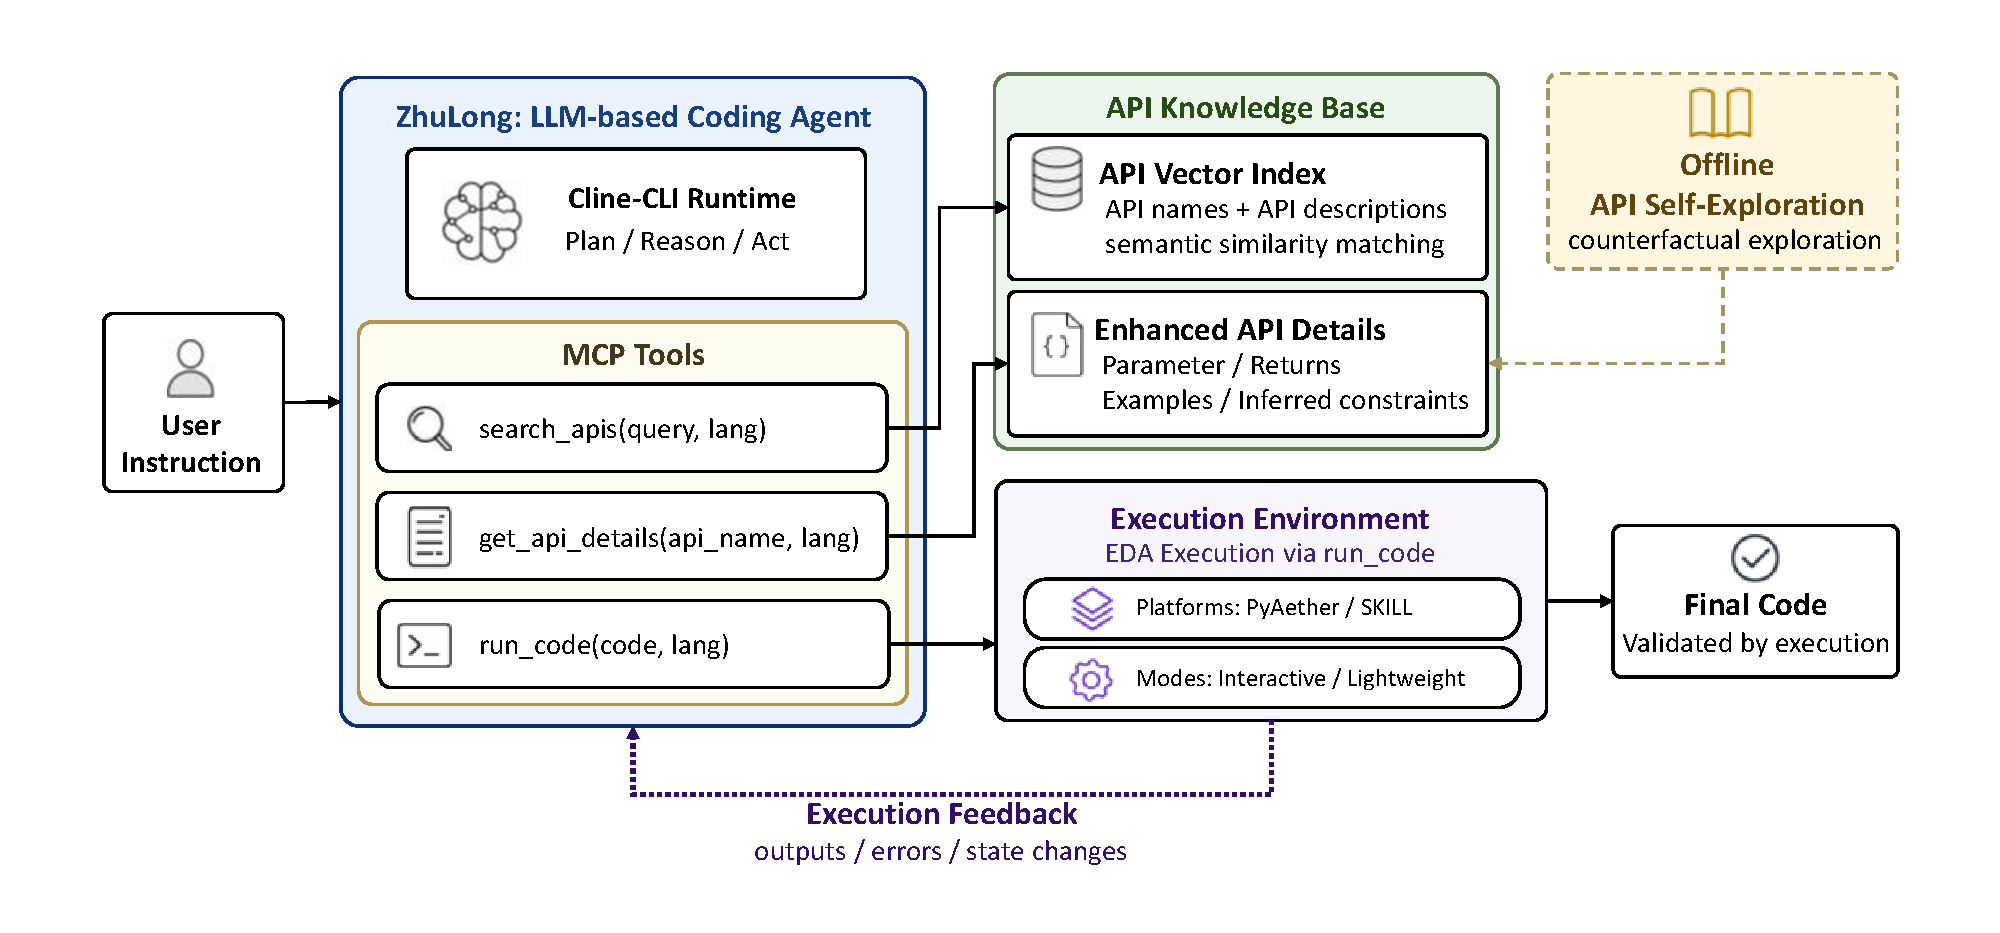
\includegraphics[width=0.9\textwidth]{figures/zhulong_arch_1.pdf}
\caption{ZhuLong system architecture. The agent interacts with API retrieval, enhanced documentation, and EDA execution via three unified MCP tools. Offline self-exploration augments the knowledge base before runtime, and execution feedback supports iterative refinement.}
% ZhuLong系统架构。智能体通过三个统一的MCP工具与API检索、增强文档和EDA执行环境交互。离线自探索在运行前增强知识库，执行反馈支持迭代优化。
\label{fig:architecture}
\end{figure*}

\subsection{Three MCP Tools}
\label{sec:mcp-tools}

ZhuLong extends three MCP tools \cite{mcp2024protocol}, each accepting a unified \texttt{lang} parameter (\texttt{pyaether} or \texttt{skill}) to support both platforms with identical agent logic:
% ZhuLong扩展了三个MCP工具 \cite{mcp2024protocol}，每个工具接受统一的\texttt{lang}参数（\texttt{pyaether}或\texttt{skill}），以相同智能体逻辑支持两个平台：

\begin{itemize}
    \item \texttt{search\_apis(query, lang)} retrieves relevant APIs via semantic and keyword-based search. We index APIs by name and description using BGE-M3 embeddings \cite{bge2024} with FAISS \cite{douze2024faiss} for efficient similarity search, returning the top-$K$ results ($K=5$ by default) with confidence scores and descriptions.
    % \texttt{search\_apis(query, lang)}通过语义和关键词检索相关API。我们使用BGE-M3嵌入 \cite{bge2024}对API名称和描述建索引，FAISS \cite{faiss2017}支持高效相似度搜索，返回top-$K$结果（默认$K=5$），附带置信度分数和描述。
    
    \item \texttt{get\_api\_details(api\_name, lang)} fetches comprehensive documentation for a specified API, including parameter types, return values, and examples. The returned documentation is augmented by the offline API self-exploration mechanism (Section~\ref{sec:selfdoc}) when available, enriching incomplete specifications with constraints and usage patterns discovered via sandbox exploration.
    % \texttt{get\_api\_details(api\_name, lang)}获取指定API的完整文档，包括参数类型、返回值和示例。当可用时，返回的文档由离线API自探索机制（第~\ref{sec:selfdoc}节）增强，补充通过沙盒探索发现的约束和使用模式。
    
    \item \texttt{run\_code(code, lang)} executes the generated code in the EDA environment. It supports two modes: (1) \textbf{interactive}—runs inside an open EDA session via socket communication, enabling operations on unsaved layouts and schematics; (2) \textbf{lightweight}—runs in a sandboxed environment without a GUI session (standalone PythonE for PyAether, or SKILL in batch mode for Virtuoso). Both modes capture outputs, errors, and state changes for iterative refinement.
    % \texttt{run_code(code, lang)}在EDA环境中执行生成的代码。支持两种模式：（1）\textbf{交互模式}——通过socket在已打开的EDA会话内运行，支持操作未保存的版图和原理图；（2）\textbf{轻量模式}——在沙盒化环境中运行，无需GUI会话（PyAether使用独立PythonE环境，Virtuoso使用SKILL批处理模式）。两种模式均捕获输出、错误和状态变化，供迭代优化使用。
\end{itemize}

\subsection{Agent Workflow}
\label{sec:agent-workflow}

The agent iteratively refines its output through execution feedback \cite{cline2024cline}. A typical trajectory begins with reasoning over the user instruction, followed by API retrieval via \texttt{search\_apis} when needed. Candidate APIs are then inspected via \texttt{get\_api\_details}, and code is generated accordingly. The agent executes the code via \texttt{run\_code}, observes the result, and re-plans—revising the code, retrieving alternative APIs, or terminating. This loop continues until success or the agent determines further attempts are unlikely to succeed. The agent is not constrained to a fixed sequence; it may skip retrieval when it already knows the required API, or conduct multiple rounds of retrieval when initial results lack confidence.
% 智能体通过执行反馈迭代优化其输出 \cite{cline2024cline}。典型轨迹始于对用户指令的推理，需要时通过\texttt{search\_apis}检索API，然后通过\texttt{get\_api\_details}查阅候选API的文档，据此生成代码。智能体通过\texttt{run\_code}执行代码、观察结果并重规划——修改代码、检索替代API或终止。此循环持续至成功或智能体判断继续尝试不太可能成功。智能体不受固定序列约束——已知所需API时可跳过检索，初始结果置信度不足时可进行多轮检索。

\section{Offline API Self-Exploration Mechanism}
\label{sec:selfdoc}

Given incomplete API documentation in Markdown format, ZhuLong enriches it through offline counterfactual exploration in a sandbox environment. The core idea is to treat the sandbox as an executable environment for probing undocumented API behavior. For each undocumented or ambiguous aspect, ZhuLong constructs counterfactual hypotheses—e.g., whether a parameter accepts an empty list, whether a numeric argument allows negative values, or whether a return value contains a specific field—and executes targeted test scripts via \texttt{run\_code} to validate them. Execution outcomes, including successful executions, errors, exceptions, return values, and state changes, reveal actual API constraints and behaviors. The agent iteratively refines its understanding by reading available documentation, writing test scripts, observing results, and deciding what to test next and when to stop. This offline process runs once per API; the enriched documentation—capturing parameter constraints, return structures, error handling, and side effects—is stored in the API knowledge base and made available to the agent via \texttt{get\_api\_details} during future runs, incurring no runtime overhead.
% 给定一份不完整的Markdown格式API文档，ZhuLong通过在沙盒环境中进行离线反事实探索来增强该文档。核心思想是将沙盒视为一个可执行环境，用于探测未文档化的API行为。对于每个未文档化或含糊的方面，ZhuLong构造反事实假设——例如参数是否接受空列表、数值参数是否允许负值、或返回值是否包含某个特定字段——并通过\texttt{run\_code}执行有针对性的测试脚本来验证这些假设。执行结果，包括成功执行、错误、异常、返回值和状态变化，揭示API的真实约束和行为。智能体通过读取已有文档、编写测试脚本、观察结果，并自主决定下一步测试什么以及何时停止，来迭代地完善其理解。该离线过程每个API运行一次；增强后的文档——包含参数约束、返回值结构、错误处理和副作用——被存储到API知识库中，并在未来运行时通过\texttt{get\_api\_details}提供给智能体，不产生运行时开销。

\section{Benchmark Construction}
\label{sec:benchmark}

\subsection{Dataset: EDA-Eval-PyAether}

To evaluate LLM-based code generation for PyAether, we constructed \textbf{EDA-Eval-PyAether}, a benchmark of 158 tasks. Tasks were collected from four sources: PyAether API references (61.4\%), official documentation examples (27.2\%), internal training materials (7.6\%), and anonymized CAD practical cases (3.8\%). Each task underwent manual review by EDA domain experts.
% 为了评估基于LLM的PyAether代码生成，我们构建了\textbf{EDA-Eval-PyAether}评测集，包含158个任务。任务收集自四个来源：PyAether API参考文档（61.4\%）、官方文档示例（27.2\%）、内部培训材料（7.6\%）和脱敏的CAD实际案例（3.8\%）。每个任务均由EDA领域专家进行了人工审核。

Table~\ref{tab:scenario-distribution} shows the distribution of tasks across different EDA scenarios. Layout and Schematic operations constitute the majority (70.2\%), reflecting the core focus of PyAether usage in physical design workflows.
% 表~\ref{tab:scenario-distribution}展示了任务在不同EDA场景中的分布。Layout和Schematic操作占大多数（70.2\%），反映了PyAether在物理设计工作流中的核心使用场景。


\begin{table}[htbp]
\centering
\caption{Task distribution by scenario}
\label{tab:scenario-distribution}
\begin{tabular}{lcc}
\toprule
\textbf{Scenario} & \textbf{Tasks} & \textbf{Percentage} \\
\midrule
Layout & 64 & 40.5\% \\
Schematic & 47 & 29.7\% \\
Design Management & 24 & 15.2\% \\
Others & 23 & 14.6\% \\
\midrule
Total & 158 & 100\% \\
\bottomrule
\end{tabular}
\end{table}
% 表：按场景划分的任务分布。

\subsection{Evaluation Protocol}

Each task consists of: (1) a natural language prompt describing the desired operation, (2) a function signature, and (3) assertion-based test code. A task is considered \textbf{passed} if the generated code executes in the PyAether sandbox without errors and all assertions evaluate to true. The primary metric is \textbf{Pass@1} \cite{chen2021evaluating}, which is equivalent to the pass rate:
% 评估协议。每个任务包含三个部分：（1）描述所需操作的自然语言提示，（2）函数签名，以及（3）基于断言的测试代码。如果生成的代码在PyAether沙盒中无错误执行且所有断言均为真，则该任务被视为\textbf{通过}。主要指标为\textbf{Pass@1} \cite{chen2021evaluating}，等同于通过率：

\[
\text{Pass@1} = \frac{\text{\# tasks with all assertions passed}}{\text{Total tasks}} \times 100\%
\]
% \[
% \text{通过率} = \frac{\text{所有断言均通过的任务数}}{\text{总任务数}} \times 100\%
% \]

\section{Experiments}
\label{sec:experiments}

\subsection{Experimental Setup}
\label{sec:exp-setup}

\subsubsection{Research Questions}

This evaluation aims to answer four research questions: (RQ1) whether sandbox execution improves code generation accuracy over static generation; (RQ2) how effectively the self-exploration mechanism handles undocumented or incomplete APIs; (RQ3) whether vector-based retrieval outperforms grep-based keyword search for API discovery; and (RQ4) how different index construction strategies affect retrieval effectiveness.
% 本评估旨在回答四个研究问题：(RQ1) 沙盒执行相比静态生成是否提升了代码生成准确率；(RQ2) 自探索机制对未文档化或不完整API的效果如何；(RQ3) 向量检索在API发现上是否优于grep关键词搜索；(RQ4) 不同的索引构建策略如何影响检索效果。

\subsubsection{Benchmark and Evaluation Protocol}

We evaluate ZhuLong on \textbf{EDA-Eval-PyAether}, a benchmark of 158 real-world PyAether scripting tasks. Following the evaluation protocol defined in Section~\ref{sec:benchmark}, we adopt \textbf{Pass@1} (execution success rate) as the primary metric. During evaluation, the agent is allowed up to \textbf{2 re-planning rounds} per task (i.e., up to three execution attempts total), following the self-correction loop described in Section~\ref{sec:agent-workflow}; timeout is set to 2500 seconds per execution.
% 评测集与评估协议。我们在\textbf{EDA-Eval-PyAether}上评估ZhuLong，该评测集包含158个真实PyAether脚本任务。遵循第\ref{sec:benchmark}节定义的评估协议，我们采用\textbf{Pass@1}（执行成功率）作为主要指标。评估过程中，智能体在每个任务上允许最多\textbf{2轮重新规划}（即最多共3次执行机会），遵循第\ref{sec:agent-workflow}节描述的自校正循环；每次执行超时时间设为2500秒。

\subsubsection{Baselines and ZhuLong Variants}

To isolate the contribution of each component, we establish two baselines and three ZhuLong variants, as shown in Table~\ref{tab:configurations}. ZhuLong variants default to vector retrieval using a name+description index.
% 基线与ZhuLong变体。为了隔离每个组件的贡献，我们建立了两个基线和三个ZhuLong变体，如表~\ref{tab:configurations}所示。ZhuLong变体默认使用名称+描述索引进行向量检索。

\begin{table}[htbp]
\centering
\caption{Configurations and their components}
\label{tab:configurations}
\begin{tabular}{lccc}
\toprule
\textbf{Configuration} & \textbf{Retrieval} & \textbf{Sandbox} & \textbf{Self-Expl.} \\
\midrule
Baseline 1 (Pure LLM) & \ding{55} & \ding{55} & \ding{55} \\
Baseline 2 (RAG) & \ding{51} & \ding{55} & \ding{55} \\
ZhuLong w/o Self-Expl. & \ding{51} & \ding{51} & \ding{55} \\
ZhuLong w/o Sandbox & \ding{51} & \ding{55} & \ding{51} \\
ZhuLong w/o Retrieval & \ding{55} & \ding{51} & \ding{51} \\
\textbf{ZhuLong} (Full) & \ding{51} & \ding{51} & \ding{51} \\
\bottomrule
\end{tabular}
\end{table}
% 表：配置及其组件。ZhuLong（完整）为完整系统，其余为消融变体。
% Self-Expl. = Self-Exploration mechanism.

\subsubsection{LLM Backbones}

All main experiments use DeepSeek-V4-Flash as the primary backbone. To understand the impact of different LLMs, we additionally evaluate DeepSeek-V3.2, GLM-5.1, DeepSeek-V4-Pro, Kimi-K2.6, and Doubao-Seed-2.0-Pro.
% LLM主干。所有主要实验使用DeepSeek-V4-flash作为主要主干。为了解不同LLM的影响，我们还评估了DeepSeek-V3.2、GLM-5.1、DeepSeek-V4-Pro、Kimi-K2.6和Doubao-Seed-2.0-Pro。

\subsubsection{Iteration Budget}
\label{sec:iteration-budget}

To understand how the agent's autonomous refinement capability contributes 
to task success, we conduct a controlled ablation on the maximum number of 
iterative correction rounds allowed per task.
% 为了理解智能体自主修正能力对任务成功的贡献，我们对每个任务允许的最大迭代
% 修正轮数进行了受控消融实验。
We evaluate three configurations: (i) a single attempt with no opportunity 
for re-planning (\textit{0 iterations}), (ii) one re-planning round 
following execution feedback (\textit{1 iteration}), and (iii) two 
re-planning rounds (\textit{2 iterations}), which corresponds to the full 
ZhuLong system configuration.
% 我们评估三种配置：（i）单次尝试，无重新规划机会（0次迭代），（ii）在执行
% 反馈后进行一轮重新规划（1次迭代），（iii）两轮重新规划（2次迭代），这对应
% 于完整的ZhuLong系统配置。
Each iteration follows the closed-loop workflow described in 
Section~\ref{sec:agent-workflow}: the agent executes code via 
\texttt{run\_code}, observes the result, and autonomously decides whether 
to revise the code, retrieve alternative APIs, or terminate.
% 每轮迭代遵循第\ref{sec:agent-workflow}节描述的闭环工作流：智能体通过
% \texttt{run\_code}执行代码，观察结果，并自主决定是修改代码、检索替代API
% 还是终止。
This design isolates the value of iterative execution feedback from the 
agent's internal reasoning, independent of any external script-level retry 
mechanism.
% 此设计将迭代执行反馈的价值与智能体内部推理分离开来，独立于任何外部的脚本
% 级重试机制。

\subsection{Main Results and Ablation}
\label{sec:exp-results}

Table~\ref{tab:main-ablation} presents the progressive build-up (top), the 
iteration budget ablation (middle), and the component ablation (bottom). 
The top and bottom blocks report the same set of configurations---all with 
2 re-planning rounds---viewed from complementary directions: the top block 
shows sequential gains as components are incrementally added (each row's 
gain is relative to the previous row), while the bottom block shows 
degradation from removing each component from the full system. The middle 
block isolates the effect of the re-planning budget itself, comparing 0, 1, 
and 2 rounds within the full system.
% 表~\ref{tab:main-ablation}呈现了渐进构建（上）、迭代预算消融（中）
% 和组件消融（下）。上和下两块报告的是同一组配置——均为2轮重新规划——
% 但从互补方向观察：上块显示组件逐步添加时各步骤的边际增益（每行增益
% 相对于上一行），下块显示从完整系统中移除各组件后的性能下降。中块则
% 分离了重新规划预算本身的影响，在完整系统内比较0、1、2轮重新规划。

\begin{table}[htbp]
\centering
\caption{Ablation study results}
\label{tab:main-ablation}
\begin{tabular}{lcc}
\toprule
\textbf{Configuration} & \textbf{Pass@1 (\%)} & \textbf{$\Delta$} \\
\midrule
\multicolumn{3}{l}{\textit{Progressive build-up (vs. previous row)}} \\
Baseline 1: Pure LLM & 23.6 & — \\
Baseline 2: RAG & 32.3 & +8.7 pp \\
ZhuLong w/o Self-Expl. & 75.3 & +43.0 pp \\
\textbf{ZhuLong} (Full) & \textbf{78.5} & \textbf{+3.2 pp} \\
\midrule
\multicolumn{3}{l}{\textit{Iteration budget ablation (vs. ZhuLong Full)}} \\
0 re-planning rounds (single attempt) & 62.7 & -15.8 pp \\
1 re-planning round & 76.0 & -2.5 pp \\
\midrule
\multicolumn{3}{l}{\textit{Component ablation (vs. ZhuLong Full)}} \\
ZhuLong w/o Self-Expl. & 75.3 & -3.2 pp \\
ZhuLong w/o Sandbox & 37.3 & -41.2 pp \\
ZhuLong w/o Retrieval & 34.2 & -44.3 pp \\
\bottomrule
\end{tabular}
\end{table}
% 表：性能构建、迭代预算消融与组件消融研究。上块为渐进构建，"Gain"表示
% 相对于前一行的增量（均为2轮重新规划）；中块为迭代预算消融，下块为组件消融，
% 中块和下块中的"Drop"均表示相对于ZhuLong完整系统（加粗行）的减量。

\subsubsection{Effect of Iteration Budget}
\label{sec:iteration-budget-effect}

The iteration budget ablation in the middle block of 
Table~\ref{tab:main-ablation} quantifies the impact of autonomous 
re-planning rounds on task success. With no re-planning opportunity (0 
iterations), ZhuLong achieves 62.7\% Pass@1—substantially higher than the 
32.3\% RAG baseline—indicating that even a single execution trace provides 
valuable signal for code generation. Allowing one re-planning round raises 
accuracy to 76.0\%, a gain of 13.3 percentage points that accounts for 
\textbf{84.2\%} of the total improvement achievable within two iterations 
(from 62.7\% to 78.5\%). The second re-planning round yields only a 
marginal 2.5 pp gain, bringing the final accuracy to 78.5\%.
% 表~\ref{tab:main-ablation} 中块的迭代预算消融量化了自主重新规划轮数
% 对任务成功的影响。无重新规划机会（0次迭代）时，ZhuLong达到62.7\%的
% Pass@1——显著高于32.3\%的RAG基线——表明单次执行轨迹已为代码生成提供了
% 有价值的信息。允许一轮重新规划将准确率提升至76.0\%，增益13.3个百分点，
% 占两轮迭代内（从62.7\%到78.5\%）可实现总提升的\textbf{84.2\%}。第二轮
% 重新规划仅带来2.5个百分点的边际增益，将最终准确率推至78.5\%。

This diminishing-return pattern suggests that most recoverable errors—parameter mismatches, missing arguments, and state precondition violations—are diagnosed and corrected within one re-planning round. The remaining failures after two iterations involve complex multi-step dependencies or implicit domain conventions that cannot be resolved from the immediate error message alone.
% 这种边际递减规律表明，大多数可恢复错误——参数不匹配、缺少参数和状态前置条件违例——能够在一个重新规划轮次内被诊断并修正。两轮迭代后剩余的失败涉及复杂多步依赖或隐式领域约定，无法仅通过即时错误信息解决。

Based on this observation, we set two re-planning rounds as the default 
configuration for all main experiments—a decision that balances accuracy 
gain against computational overhead, and is justified by the clear 
diminishing returns observed empirically.
% 基于这一观察，我们将两轮重新规划设为所有主实验的默认配置——这一决策
% 在准确率增益与计算开销之间取得了平衡，且得到了经验观察中明显的边际
% 收益递减规律的支持。

\subsubsection{Effect of Sandbox Execution (RQ1)}

Sandbox execution is the dominant performance driver. Adding it to the RAG baseline raises Pass@1 from 32.3\% to 75.3\%---a gain of \textbf{43.0 percentage points} that accounts for \textbf{78.3\%} of the total improvement from Pure LLM (23.6\%) to ZhuLong (78.5\%). Conversely, removing sandbox execution from ZhuLong drops Pass@1 to 37.3\%, a decline of \textbf{41.2 percentage points}. These results confirm that execution feedback is indispensable: without it, the agent cannot verify correctness, observe API behavior, or iteratively refine its output.
% 沙盒执行的效果（RQ1）。沙盒执行是性能提升的主导因素。将其加入RAG基线后，Pass@1从32.3\%提升至75.3\%——增益\textbf{43.0个百分点}，占从Pure LLM（23.6\%）到ZhuLong（78.5\%）总提升的\textbf{78.3\%}。相反，从ZhuLong中移除沙盒执行后，Pass@1降至37.3\%，下降了\textbf{41.2个百分点}。这些结果确认了执行反馈不可或缺：没有它，智能体无法验证正确性、观察API行为或迭代优化其输出。

We attribute this to two mechanisms. First, execution provides concrete error messages that guide corrections, transforming one-shot generation into iterative search. Second, the agent can experiment with parameter combinations in the sandbox, compensating for gaps in documentation \cite{kumar2026agentforge, jiang2024seed}.
% 我们将此归因于两种机制。第一，执行提供具体的错误信息引导修正，将一次性生成转化为迭代搜索。第二，智能体可以在沙盒中尝试不同的参数组合，弥补文档中的不足。

\subsubsection{Effect of Self-Exploration (RQ2)}

Removing the self-exploration mechanism (while keeping sandbox execution and retrieval) reduces Pass@1 from ZhuLong's 78.5\% to 75.3\%, a drop of 3.2 percentage points. This confirms that the self-exploration mechanism---the defining component of ZhuLong---contributes a measurable accuracy gain.
% API自探索的效果（RQ2）。移除自探索机制（同时保留沙盒执行和检索）使Pass@1从ZhuLong的78.5\%降至75.3\%，下降3.2个百分点。这确认了API自探索机制——ZhuLong的定义性组件——贡献了可测量的准确率提升。

Beyond accuracy, the self-exploration mechanism also improves efficiency. Table~\ref{tab:selfdoc-efficiency} compares tool usage with and without self-exploration. With self-exploration enabled (i.e., ZhuLong), the agent produces more traces (243 vs. 220) because it persists longer with better documentation, yet total tool calls drop by 13.9\% and average calls per trace decrease by 22.1\%.
% 除了准确率，API自探索还提升了效率。表~\ref{tab:selfdoc-efficiency}比较了启用和未启用API自探索时的工具使用情况。启用API自探索后（即ZhuLong），智能体产生了更多的轨迹（243对220），因为更好的文档使其更持久地尝试，但总工具调用次数下降了13.9\%，每次轨迹的平均调用次数下降了22.1\%。

\begin{table}[htbp]
\centering
\caption{Overall tool usage: with vs. without self-exploration}
\label{tab:selfdoc-efficiency}
\begin{tabular}{lcc}
\toprule
\textbf{Metric} & \textbf{w/o Self-Expl.} & \textbf{ZhuLong (Full)} \\
\midrule
Traces & 220 & 243 (+10.5\%) \\
\#Calls & 6,791 & 5,845 (-13.9\%) \\
Avg/Trace & 30.9 & 24.1 (-22.1\%) \\
\midrule
Change & — & \textbf{-946 (-13.9\%)} \\
\bottomrule
\end{tabular}
\end{table}
% 表：整体工具使用情况：启用与未启用API自探索的对比。

The reduction is most pronounced in \texttt{run\_code} (27.0\%, see Table~\ref{tab:tool-breakdown}), indicating that enriched documentation reduces trial-and-error executions. Calls to \texttt{search\_apis} decrease by 12.2\%, while \texttt{get\_api\_details} increase by 9.0\%---a behavioral shift toward more thorough reading before coding.
% \texttt{run\_code}的降幅最为显著（27.0\%），表明增强后的文档减少了试错执行。\texttt{search\_apis}调用下降12.2\%，而\texttt{get\_api\_details}增加9.0\%——这是一种行为转变，即在编码前更充分地阅读文档。

\begin{table}[htbp]
\centering
\caption{Tool-wise call count breakdown}
\label{tab:tool-breakdown}
\begin{tabular}{lcc}
\toprule
\textbf{Tool} & \textbf{w/o Self-Expl.} & \textbf{ZhuLong (Full)} \\
\midrule
\texttt{search\_apis} & 3,203 & 2,812 (-12.2\%) \\
\texttt{get\_api\_details} & 1,151 & 1,255 (+9.0\%) \\
\texttt{run\_code} & 2,437 & 1,778 (-27.0\%) \\
\bottomrule
\end{tabular}
\end{table}
% 表：各工具调用次数明细。

In the absence of sandbox execution, the self-exploration mechanism alone improves Pass@1 from 32.3\% (RAG) to 37.3\% (ZhuLong w/o Sandbox), a gain of 5.0 percentage points. This confirms that enhanced documentation improves generation accuracy even without iterative refinement. The larger gain in the no-sandbox setting (5.0 pp vs. 3.2 pp in ZhuLong) suggests that sandbox execution partially substitutes for pre-explored documentation.
% 在没有沙盒执行的情况下，仅靠API自探索将Pass@1从32.3\%（RAG）提升至37.3\%（ZhuLong w/o Sandbox），增益5.0个百分点。这确认了增强后的文档即使在没有迭代优化的情况下也能提升生成准确率。无沙盒设置下的更大增益（5.0 pp对比ZhuLong中的3.2 pp）表明沙盒执行在一定程度上替代了预探索文档的需求。

\subsubsection{Retrieval Strategy (RQ3) and Index Construction (RQ4)}

Vector-based semantic retrieval outperforms grep-based keyword search by 12.7 percentage points (78.5\% vs. 65.8\%), confirming that natural language queries for EDA tasks rarely match exact API names. For index construction, the name+description index achieves the best result (78.5\%), outperforming description-only (76.0\%) and name-only (75.3\%), indicating that names enable exact matching while descriptions support semantic generalization. Prompt language (English vs. Chinese) shows no material difference, both achieving 78.5\% Pass@1.
% 检索策略（RQ3）与索引构建（RQ4）。基于向量的语义检索比基于grep的关键词搜索高出12.7个百分点（78.5\%对比65.8\%），确认了EDA任务的自然语言查询很少能精确匹配API名称。在索引构建方面，名称+描述联合索引取得了最佳结果（78.5\%），优于仅描述索引（76.0\%）和仅名称索引（75.3\%），表明名称支持精确匹配，而描述支持语义泛化。提示语言（英文 vs. 中文）没有实质性差异，两者均达到78.5\%的Pass@1。

\subsubsection{Impact of LLM Backbone}

Table~\ref{tab:llm-comparison} presents the Pass@1 results for six LLM backbones integrated into the full ZhuLong system. We adopt DeepSeek‑V4‑Flash as the primary backbone across all experiments in this paper, based on a practical trade‑off between model capability and inference cost: its performance is sufficiently strong to support the key findings from both our main experiments and ablation studies, while its cost remains manageable for running the complete set of configurations reported in this work. Kimi‑K2.6 achieves the highest accuracy (83.5\%), outperforming DeepSeek‑V4‑Flash (78.5\%) by 5.0 percentage points. DeepSeek‑V4‑Pro also surpasses this baseline, reaching 81.0\% (+2.5 pp), while GLM‑5.1 ties with DeepSeek‑V4‑Flash at 78.5\%. In contrast, DeepSeek‑V3.2 and Doubao‑Seed‑2.0‑Pro lag notably behind, yielding 67.1\% and 55.7\%, respectively. The spread of 27.8 percentage points between the best and worst performers indicates that the underlying model remains a decisive factor, even with retrieval, sandbox, and self‑exploration in place. Notably, the ranking on this benchmark does not strictly follow the general coding proficiency reported in public leaderboards. This discrepancy suggests that EDA scripting—with its long‑tail APIs and state‑sensitive logic—imposes a distinct set of demands that generic code benchmarks do not adequately capture.
%表~\ref{tab:llm-comparison} 给出了六个LLM主干在完整ZhuLong系统上的Pass@1结果。我们选择DeepSeek‑V4‑flash作为本文所有实验的主干模型，主要基于模型能力与推理成本之间的实际均衡考量：其性能足以支撑主实验和消融实验的核心结论，同时计算开销也在可控范围内，便于完整运行本文报告的全部实验配置。Kimi‑K2.6表现最佳（83.5%），较DeepSeek‑V4‑flash（78.5%）高出5.0个百分点。DeepSeek‑V4‑pro同样超过该基线，达到81.0%（+2.5 pp），而GLM‑5.1与DeepSeek‑V4‑flash持平，同为78.5%。相比之下，DeepSeek‑V3.2和Doubao‑Seed‑2.0‑Pro明显落后，分别为67.1%和55.7%。最好与最差模型之间相差27.8个百分点，说明即便配备了检索、沙盒和自探索机制，基座模型的选择依然是决定性能的关键因素。值得注意的是，这些模型在此评测上的排序与通用代码生成榜单并不完全一致，这一偏差表明EDA脚本任务因其长尾API和状态敏感逻辑，对LLM提出了通用基准测试难以覆盖的独特要求。

\begin{table}[htbp]
\centering
\caption{Impact of LLM backbone (ZhuLong)}
\label{tab:llm-comparison}
\begin{tabular}{lcc}
\toprule
\textbf{LLM Backbone} & \textbf{Pass@1 (\%)} & \textbf{$\Delta$} \\
\midrule
DeepSeek-V4-Flash & 78.5 & — \\
GLM-5.1 & 78.5 & — \\
DeepSeek-V3.2 & 67.1 & -11.4 pp \\
DeepSeek-V4-Pro & 81.0 & +2.5 pp \\
Kimi-K2.6 & 83.5 & +5.0 pp \\
Doubao-Seed-2.0-Pro & 55.7 & -22.8 pp \\
\bottomrule
\end{tabular}
\end{table}
% 表：LLM主干的影响（ZhuLong）。

\subsection{Error Analysis}
\label{sec:exp-error}

We analyzed the 34 failed cases from ZhuLong with DeepSeek-V4-Flash. As shown in Table~\ref{tab:error-classification}, 38.2\% of failures are generation-level (dominated by timeout, 32.4\%) and 61.8\% are execution-level failures. The execution failures all lack explicit error messages, making root-cause diagnosis difficult; we suspect they stem from API parameter mismatches, incorrect assumptions about design database state, or unhandled runtime exceptions.
% 错误分析。我们分析了ZhuLong在DeepSeek-V4-Flash上的34个失败案例。如表~\ref{tab:error-classification}所示，38.2\%的失败是生成级别的（以超时为主，占32.4\%），61.8\%是执行级别的失败。执行失败均缺乏明确的错误信息，使得根本原因诊断困难；我们推测这些失败源于API参数不匹配、对设计数据库状态的错误假设或未处理的运行时异常。

\begin{table}[htbp]
\centering
\caption{Error classification of the 34 failed cases}
\label{tab:error-classification}
\begin{tabular}{lcc}
\toprule
\textbf{Error Category} & \textbf{Count} & \textbf{Percentage} \\
\midrule
Generation timeout & 11 & 32.4\% \\
Generation fail & 2 & 5.9\% \\
Execution failure & 21 & 61.8\% \\
\midrule
Total & 34 & 100\% \\
\bottomrule
\end{tabular}
\end{table}
% 表：34个失败案例的错误分类。

The prevalence of execution-level failures underscores the need for finer-grained runtime instrumentation in future sandbox designs to enable precise failure attribution.
% 执行级失败的普遍性凸显了在未来沙盒设计中需要更细粒度的运行时检测，以实现精确的失败归因。

\subsection{Interactive Scenario Evaluation}
\label{sec:exp-interactive}

Beyond standalone execution tasks, real-world EDA scripting often involves direct manipulation of unsaved layouts and schematics. To assess ZhuLong in such GUI-bridged scenarios, we collected 20 tasks requiring operation on volatile in-memory states, window focus handling, and GUI-level interactions. All tasks were executed via the interactive mode of \texttt{run\_code} with a single attempt (no retry), as the iterative recovery loop is not supported in the bridge-based environment. These evaluations were conducted with self-exploration disabled; results thus reflect ZhuLong w/o Self-Exploration in interactive settings.
% 除了沙盒中的独立执行任务外，真实世界的EDA脚本编写通常还涉及对未保存版图和原理图的直接操作。为了评估ZhuLong在此类GUI桥接场景中的能力，我们收集了20个要求操作易变内存状态、处理窗口焦点和GUI级交互的任务。所有任务均通过\texttt{run\_code}的交互模式执行，单次尝试（无重试），因为桥接环境不支持迭代恢复循环。这些评估在禁用自探索的情况下进行，结果反映的是ZhuLong w/o Self-Exploration在交互场景中的表现。

Table~\ref{tab:interactive-results} shows the results across the same 20 tasks for both PyAether and SKILL. The overall Pass@1 is \textbf{60.0\%} for PyAether and \textbf{50.0\%} for SKILL—notably lower than the 78.5\% achieved on the main benchmark. This gap is attributed to two factors: (1) no iterative recovery loop, limiting each task to a single attempt; and (2) self-exploration disabled. Performance varies by task category: PyAether excels in focus-dependent and modification tasks (75.0\% or higher), while SKILL shows an advantage in design content manipulation and hierarchical inspection. Focus-dependent operations are the most challenging for SKILL (25.0\%), while design content manipulation is the most difficult for PyAether (37.5\%). The 10~pp overall gap reflects Python's more favorable syntax for LLM-based synthesis compared to SKILL's Lisp-based prefix notation.
% 表~\ref{tab:interactive-results}展示了PyAether和SKILL在相同20个任务上的结果。PyAether的整体Pass@1为60.0\%，SKILL为50.0\%——明显低于主评测集的78.5\%。这一差距可归因于两个因素：（1）无迭代恢复循环，每个任务仅限单次尝试；（2）自探索未启用。不同任务类别的表现差异显著：PyAether在焦点依赖和修改类任务中表现优异（75.0\%以上），SKILL在设计内容操作和层次化检查方面相对占优。焦点依赖操作对SKILL最具挑战性（25.0\%），而对PyAether而言设计内容操作难度最大（37.5\%）。10个百分点的整体差距反映了Python语法对LLM合成更为友好。

\begin{table}[htbp]
\centering
\caption{Interactive scenario results: same 20 tasks for PyAether and SKILL}
\label{tab:interactive-results}
\begin{tabular}{lccc}
\toprule
\textbf{Category} & \textbf{Tasks} & \textbf{PyAether} & \textbf{SKILL} \\
\midrule
Design content manipulation & 8 & 37.5\% & 50.0\% \\
Focus-dependent operations & 4 & 75.0\% & 25.0\% \\
Hierarchical inspection & 4 & 50.0\% & 75.0\% \\
Design modification & 2 & 100.0\% & 50.0\% \\
GUI interaction & 2 & 100.0\% & 50.0\% \\
\midrule
Overall & 20 & 60.0\% & 50.0\% \\
\bottomrule
\end{tabular}
\end{table}
% 表：交互场景任务分布与结果。

\section{Discussion}
\label{sec:discussion}

\subsection{Failure Case Analysis}

Despite the improvements, ZhuLong still fails on certain cases. We identify three typical failure modes:

\textbf{Complex multi-step logic.} Tasks with conditional branches or loops often fail, consistent with the "constraint decay" phenomenon where performance declines as structural requirements accumulate \cite{dente2026constraint}. The agent struggles with state management across steps, a limitation that stems from the underlying LLM's reasoning capability rather than component absence.
% \textbf{复杂多步逻辑。} 包含条件分支或循环的任务经常失败，这与"约束衰减"现象一致，即结构性要求累积时性能下降 \cite{dente2026constraint}。智能体在多步状态管理上存在困难，这一限制源于底层LLM的推理能力而非组件缺失。

\textbf{Domain-specific conventions.} Implicit conventions (e.g., coordinate systems, layer naming) are known to experienced designers but documented nowhere. Even with self-exploration enabled, ZhuLong cannot infer conventions entirely absent from both documentation and codebase \cite{jiang2024seed}.
% \textbf{领域特定惯例。} 隐式约定（如坐标系、图层命名）对有经验的设计师是常识，但无文档记载。即使启用了自探索，ZhuLong也无法推断完全不存在于文档和代码库中的约定 \cite{jiang2024seed}。

\textbf{Environment state sensitivity.} In interactive scenarios (60\% Pass@1 on 20 cases), the agent must handle unsaved windows, focus states, and user confirmations—dynamic states hard to capture in a sandbox. Enabling self-exploration in interactive settings remains future work.
% \textbf{环境状态敏感性。} 在交互场景中（20个任务上60\% Pass@1），智能体需处理未保存窗口、焦点状态和用户确认——这些动态状态在沙盒中难以捕获。在交互式环境中启用自探索仍是未来工作。

\subsection{Limitations}

ZhuLong has four main limitations. First, performance varies significantly across base LLMs, from 83.5\% (Kimi-K2.6) to 55.7\% (Doubao-Seed-2.0-Pro) \cite{sharifloo2025struggle}. Second, offline self-exploration incurs upfront cost (one-time sandbox execution per API), amortized over subsequent queries. Third, the interactive bridge has concurrency limitations due to single-threaded daemon execution. Fourth, the benchmark, while realistic, is limited to 158 cases.
% ZhuLong有四个主要限制。第一，不同基座LLM表现差异显著，从83.5\%（Kimi-K2.6）到55.7\%（Doubao-Seed-2.0-Pro）不等 \cite{sharifloo2025struggle}。第二，离线自探索需预先计算成本（每个API一次沙盒执行），在后续查询中被摊销。第三，交互桥接因单线程守护进程存在并发限制。第四，评测集虽真实但仅限于158个案例。

\subsection{Broader Implications}

Our findings suggest that sandbox execution and offline self-exploration may generalize to other domain-specific code generation tasks with similar characteristics—long-tailed APIs, incomplete documentation, and available execution feedback \cite{kumar2026agentforge}. The architecture may transfer with minimal adaptation, though self-exploration must be re-targeted to each new API ecosystem.
% 更广泛的影响。我们的发现表明，沙盒执行和离线自探索可能推广到其他具有相似特征的领域特定代码生成任务——长尾API、文档不完整且有执行反馈可用 \cite{kumar2026agentforge}。该架构可最小适配迁移，但自探索需针对每个新API生态系统重新定制。

\section{Conclusion and Future Work}
\label{sec:conclusion}

This paper presents \textbf{ZhuLong}, an LLM-based coding agent that grounds EDA script generation in execution feedback via sandbox execution and an offline API self-exploration mechanism. The complete system achieves 78.5\% Pass@1 on our EDA-Eval-PyAether benchmark of 158 real-world tasks. Our ablation studies reveal a key insight: execution feedback is the dominant performance driver, while self-exploration contributes both accuracy gains and measurable efficiency improvements by reducing trial-and-error tool calls. These findings demonstrate that, for domain-specific scripting with long-tail, under-documented APIs, grounding generation in execution and proactive API exploration is far more effective than relying on static knowledge alone. Code and benchmark will be released upon acceptance.
% 本文提出\textbf{ZhuLong}，一个将EDA脚本生成建立在执行反馈之上的LLM智能体，通过沙盒执行和离线API自探索机制实现。完整系统在我们的EDA-Eval-PyAether评测集（158个真实任务）上达到78.5\%的Pass@1。消融实验揭示了一个关键洞察：执行反馈是性能提升的主导因素，而API自探索在带来准确率提升的同时，通过减少试错调用显著提高了效率。这些发现表明，面对长尾、文档不完善的领域特定脚本任务，将生成建立在执行和主动API探索之上，远比仅依赖静态知识更为有效。代码和评测集将在录用后开源。

Future work includes multimodal integration for layout and schematic understanding, self-evolution through continuous learning from successful and failed cases, code-to-iflow conversion for automated workflow deployment, systematic expansion of the interactive benchmark to cover diverse GUI operations and volatile environment states, and extension to additional EDA platforms such as Synopsys tools with Tcl scripting.
% 未来工作包括：多模态集成用于版图和原理图理解，通过成功与失败案例持续学习的自我进化，代码到iflow转换实现自动化工作流部署，系统性扩展交互式评测集以覆盖多样化GUI操作和易变环境状态，以及扩展至Synopsys工具Tcl脚本等其他EDA平台。

%%
%% The next two lines define the bibliography style to be used, and
%% the bibliography file.
\bibliographystyle{ACM-Reference-Format}
\bibliography{reference}

\end{document}
\endinput
%%
%% End of file `sigconf.tex'.
